\documentclass{beamer}
\mode<presentation>
\title{Free and Open Source Software}
\author{Andrea Bellandi, Alessandro Campagni}
\usetheme{CambridgeUS}


\begin{document}


\begin{frame}
  \titlepage

\vfill

\includegraphics[width=0.05\textwidth]{img/cc.png}

\includegraphics[width=0.05\textwidth]{img/by.png}

\includegraphics[width=0.05\textwidth]{img/sa.png}

This work is licensed under the Creative Commons
Attribution-ShareAlike 3.0 Unported License. 
To view a copy of this license, visit 
http://creativecommons.org/licenses/by-sa/3.0/.
\end{frame}

\begin{frame}
  \frametitle{Free and Open Source Software}

  \begin{itemize}
    \item Cosa \`e il FOSS
  \end{itemize}

\end{frame}


\begin{frame}
  \frametitle{Cosa \`e il FOSS}

  \begin{itemize}
    \item<1-> Computer, Software e schermate blu
    \item<2-> Un po' di storia
    \item<3-> Il codice sorgente
  \end{itemize}

\end{frame}


\begin{frame}
  \frametitle{Il codice sorgente}

  \begin{center}
      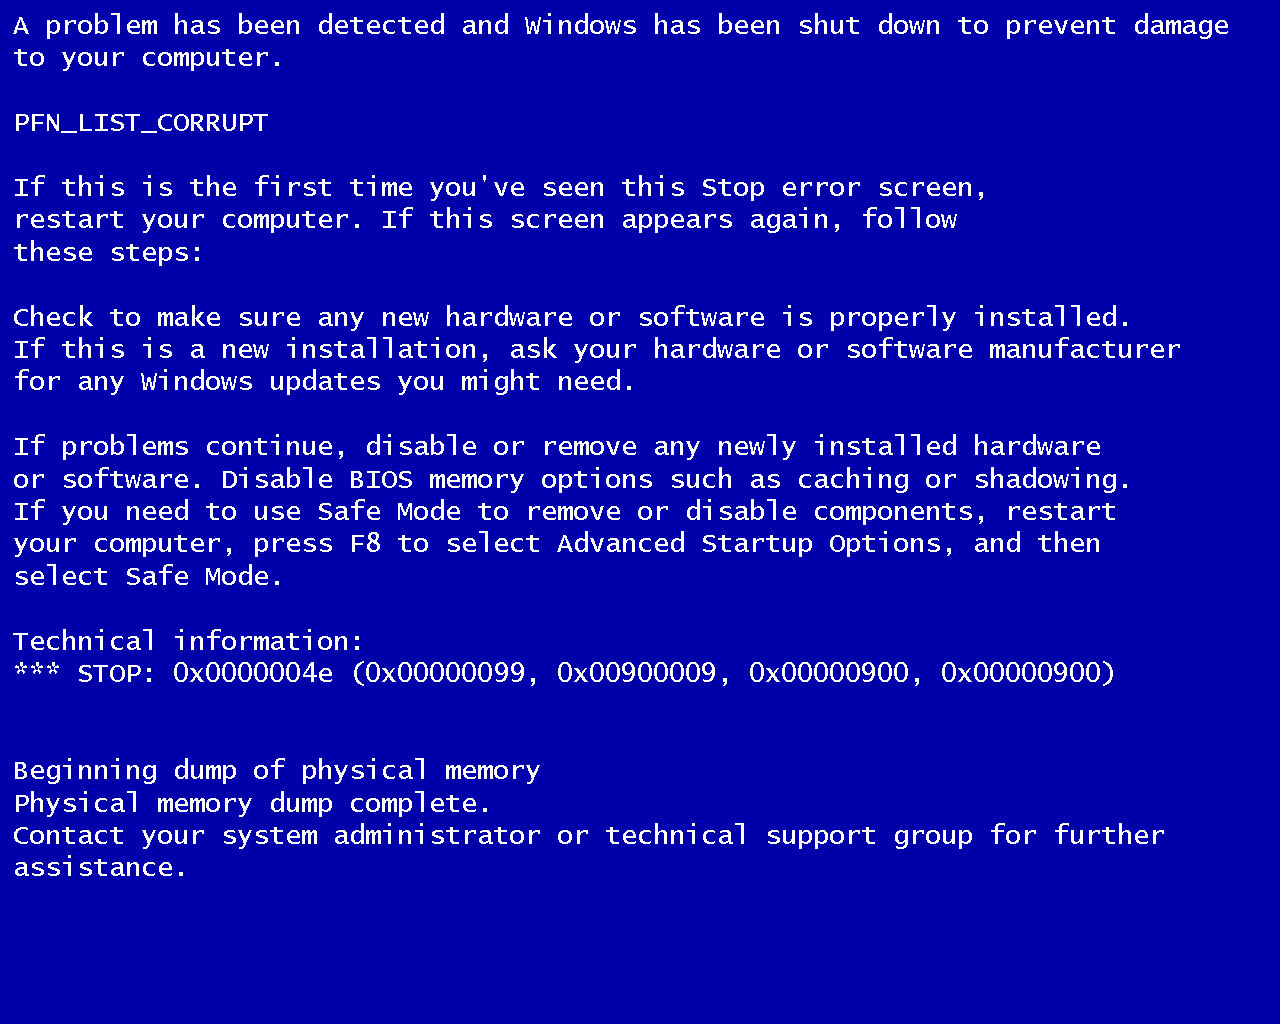
\includegraphics[width=0.7\textwidth]{img/bsod.jpg}
  \end{center}

\end{frame}


\begin{frame}
  \frametitle{Il codice sorgente}
  \fontsize{12}{7.2}\selectfont
  \begin{center}
c7 3c 2a 3c 2a 2b 2a 5c 3c 28 5c 2a 2b 2a 5c 3c\\
28 5c 2a 2b 2a 5c 3c 28 5c 2a 2b 2a 5c 3c 28 5c\\
2a 2b 2a 5c 3c 28 5c 2a 2b 2a 5c 3c 28 5c 2a 2b\\
2a 5c 3c 28 5c 2a 2b 2a 5c 3c 28 5c 2a 2b 2a 5c\\
3c 28 5c 2a 2b 2a 5c 3c 28 5c 2a 2b 2a 5c 3c 28\\
5c 2a 2b 2a 5c 3c 28 5c 2a 2b 2a 5c 3c 28 5c 2a\\
2b 2a 00 00 01 00 00 00 00 00 00 00 00 00 00 00\\
00 00 00 00 00 00 00 00 00 00 00 00 00 00 00 00\\
00 00 00 00 00 00 00 00 00 00 00 00 00 00 00 00\\
00 00 00 00 00 00 00 00 00 00 00 00 00 00 00 00\\
00 00 00 00 00 00 00 00 00 00 00 00 00 00 00 00\\
00 00 00 00 00 00 00 00 00 00 00 00 00 00 00 00\\
00 00 00 00 00 00 00 64 48 65 6c 6c 6f 2c 20 57\\
6f 72 6c 64 21 00 00 00 00 00 00 00 00 00 00 00\\
00 00 00 00 00 00 00 00 00 00 00 00 00 00 00 00\\
00 00 00 00 00 00 00 00 00 00 00 00 00 00 00 00
  \end{center}

\end{frame}


\begin{frame}[fragile]
  \frametitle{Il codice sorgente}
  
  \begin{verbatim}
#include <stdio.h>
#include <stdlib.h>

int main(int arcg, char *argv[])
{
  printf("Hello World!");
  return EXIT_SUCCESS;
}
  \end{verbatim}

\end{frame}

\begin{frame}
  \frametitle{Cosa \`e il FOSS}

  \begin{itemize}
    \item Computer, Software e schermate blu
    \item Un po' di storia
    \item Il codice sorgente
    \item Huston, abbiamo un problema
  \end{itemize}

\end{frame}


\begin{frame}
  \frametitle{Free and Open Source Software}

  \begin{itemize}
    \item Cosa \`e il FOSS
    \item Le quattro libert\`a
  \end{itemize}

\end{frame}

\begin{frame}
  \frametitle{Le quattro libert\`a}

  \begin{itemize}
    \item<1-> \emph{Libert\`a 0} Libert\`a di eseguire il programma
      per qualsiasi scopo.
    \item<2-> \emph{Libert\`a 1} Libert\`a di studiare il programma e
      modificarlo.
    \item<3-> \emph{Libert\`a 2} Libert\`a di ridistribuire copie del
      programma in modo da aiutare il prossimo.
    \item<4-> \emph{Libert\`a 3} Libert\`a di migliorare il programma e di distribuirne pubblicamente i miglioramenti, in modo tale che tutta la comunit\`a ne tragga beneficio.
  \end{itemize}

\end{frame}

\begin{frame}
  \frametitle{Free and Open Source Software}

  \begin{itemize}
    \item Cosa \`e il FOSS
    \item Le quattro libert\`a
    \item Ma allora conviene?
  \end{itemize}

\end{frame}

\begin{frame}
  \frametitle{Ma allora conviene?}
  
  \begin{center}
    SI!
  \end{center}

\end{frame}

\begin{frame}
  \frametitle{Ma allora conviene?}


  \begin{block}{I motivi della convenienza}
    
    \begin{itemize}
      \item<1-> Le quattro libert\`a
      \item<2-> Le quattro libert\`a
      \item<3-> Le quattro libert\`a
      \item<4-> Veloce risoluzione bug
      \item<5-> Indipendenza da chi produce software
      \item<6-> Facile interscambio di informazioni e dati fra le
        varie parti
      \item<7-> Adattare al meglio il programma alle proprie esigenze
    \end{itemize}

  \end{block}
  
\end{frame}


\begin{frame}
  \frametitle{Ma allora conviene?}


  \begin{block}{I motivi della convenienza}
    
    \begin{itemize}
      \item Le quattro libert\`a
      \item Le quattro libert\`a
      \item Le quattro libert\`a
      \item Veloce risoluzione bug
      \item Indipendenza da chi produce software
      \item Facile interscambio di informazioni e dati fra le
        varie parti
      \item Adattare al meglio il programma alle proprie esigenze
    \end{itemize}
  \end{block}


  \begin{block}{Un esempio}
    Ricetta o teorema?!?!
  \end{block}


\end{frame}


\end{document}
